% Options for packages loaded elsewhere
\PassOptionsToPackage{unicode}{hyperref}
\PassOptionsToPackage{hyphens}{url}
%
\documentclass[
  12pt,
]{article}
\usepackage{amsmath,amssymb}
\usepackage{lmodern}
\usepackage{iftex}
\ifPDFTeX
  \usepackage[T1]{fontenc}
  \usepackage[utf8]{inputenc}
  \usepackage{textcomp} % provide euro and other symbols
\else % if luatex or xetex
  \usepackage{unicode-math}
  \defaultfontfeatures{Scale=MatchLowercase}
  \defaultfontfeatures[\rmfamily]{Ligatures=TeX,Scale=1}
\fi
% Use upquote if available, for straight quotes in verbatim environments
\IfFileExists{upquote.sty}{\usepackage{upquote}}{}
\IfFileExists{microtype.sty}{% use microtype if available
  \usepackage[]{microtype}
  \UseMicrotypeSet[protrusion]{basicmath} % disable protrusion for tt fonts
}{}
\makeatletter
\@ifundefined{KOMAClassName}{% if non-KOMA class
  \IfFileExists{parskip.sty}{%
    \usepackage{parskip}
  }{% else
    \setlength{\parindent}{0pt}
    \setlength{\parskip}{6pt plus 2pt minus 1pt}}
}{% if KOMA class
  \KOMAoptions{parskip=half}}
\makeatother
\usepackage{xcolor}
\usepackage[margin=1in]{geometry}
\usepackage{graphicx}
\makeatletter
\def\maxwidth{\ifdim\Gin@nat@width>\linewidth\linewidth\else\Gin@nat@width\fi}
\def\maxheight{\ifdim\Gin@nat@height>\textheight\textheight\else\Gin@nat@height\fi}
\makeatother
% Scale images if necessary, so that they will not overflow the page
% margins by default, and it is still possible to overwrite the defaults
% using explicit options in \includegraphics[width, height, ...]{}
\setkeys{Gin}{width=\maxwidth,height=\maxheight,keepaspectratio}
% Set default figure placement to htbp
\makeatletter
\def\fps@figure{htbp}
\makeatother
\setlength{\emergencystretch}{3em} % prevent overfull lines
\providecommand{\tightlist}{%
  \setlength{\itemsep}{0pt}\setlength{\parskip}{0pt}}
\setcounter{secnumdepth}{-\maxdimen} % remove section numbering
\newlength{\cslhangindent}
\setlength{\cslhangindent}{1.5em}
\newlength{\csllabelwidth}
\setlength{\csllabelwidth}{3em}
\newlength{\cslentryspacingunit} % times entry-spacing
\setlength{\cslentryspacingunit}{\parskip}
\newenvironment{CSLReferences}[2] % #1 hanging-ident, #2 entry spacing
 {% don't indent paragraphs
  \setlength{\parindent}{0pt}
  % turn on hanging indent if param 1 is 1
  \ifodd #1
  \let\oldpar\par
  \def\par{\hangindent=\cslhangindent\oldpar}
  \fi
  % set entry spacing
  \setlength{\parskip}{#2\cslentryspacingunit}
 }%
 {}
\usepackage{calc}
\newcommand{\CSLBlock}[1]{#1\hfill\break}
\newcommand{\CSLLeftMargin}[1]{\parbox[t]{\csllabelwidth}{#1}}
\newcommand{\CSLRightInline}[1]{\parbox[t]{\linewidth - \csllabelwidth}{#1}\break}
\newcommand{\CSLIndent}[1]{\hspace{\cslhangindent}#1}
\usepackage{float}
\usepackage{titling}
\usepackage{graphicx}
\usepackage{booktabs}
\usepackage{longtable}
\usepackage{array}
\usepackage{multirow}
\usepackage{wrapfig}
\usepackage{float}
\usepackage{colortbl}
\usepackage{pdflscape}
\usepackage{tabu}
\usepackage{threeparttable}
\usepackage{threeparttablex}
\usepackage[normalem]{ulem}
\usepackage{makecell}
\usepackage{xcolor}
\ifLuaTeX
  \usepackage{selnolig}  % disable illegal ligatures
\fi
\IfFileExists{bookmark.sty}{\usepackage{bookmark}}{\usepackage{hyperref}}
\IfFileExists{xurl.sty}{\usepackage{xurl}}{} % add URL line breaks if available
\urlstyle{same} % disable monospaced font for URLs
\hypersetup{
  pdftitle={Comparing Weighting Methods and Likelihood-based Methods in Two-Stage Sampling Design with Varied Degree of Data Missingness},
  pdfauthor={Minghui Sun; Eric Reyes},
  hidelinks,
  pdfcreator={LaTeX via pandoc}}

\title{Comparing Weighting Methods and Likelihood-based Methods in
Two-Stage Sampling Design with Varied Degree of Data Missingness}
\author{Minghui Sun \and Eric Reyes}
\date{}

\begin{document}
\maketitle

\vspace{1cm}
\begin{center}
\textbf{Abstract}
\end{center}

Data can be lost for different reasons, but sometimes the missingness is
a part of the data collection process. Unbiased and efficient estimation
of the parameters governing the response mean model requires the missing
data to be appropriately addressed. This paper compares and contrasts
the Maximum Likelihood and Inverse Probability Weighting estimators in
an Outcome-Dependent Sampling design that deliberately generates
incomplete observations. We demonstrate the comparison through numerical
simulations under varied conditions: different coefficients of
determination, and whether or not the mean model is misspecified.

\textbf{Keyword}: Outcome-Dependent Sampling, Maximum Likelihood,
Inverse Probability Weighting, EM Algorithm \vfill

\begin{center}
{\fontsize{15}{18}\selectfont Rose-Hulman Institute of Technology}\par
{\fontsize{15}{18}\selectfont Spring, 2021}
\end{center}
\pagebreak

\hypertarget{introduction}{%
\subsection{1 Introduction}\label{introduction}}

Consider a hypothetical study about the association between oxygen
levels and the age of patients with COVID-19. Researchers may conduct it
in two stages, sampling patients' ages and oxygen levels in the first
stage. Based on the information obtained from the first stage, the
researchers identify some elderly patients to be critically ill.~Then,
in the second stage, the researcher will collect detailed information
such as medical history from these seriously ill patients. This
hypothetical study is an example of an Outcome-Dependent Sampling (ODS)
study, where data are collected in two stages. In the first stage,
information is available on the response and some of the covariates for
all observations. However, in the second stage, information is available
on other covariates among only a subset of the sample (Zhao and Lipsitz
1992). Further, the likelihood of observing an individual in the second
stage can depend on data collected during the first stage. This sampling
method allows researchers to concentrate resources on places with the
most valuable information according to their topic (Weaver and Zhou
2005). However, this unique design deliberately generates incomplete
observations in the final dataset. Therefore, estimation of the
parameters governing the model for the response requires the missing
data to be appropriately addressed.

Among applied researchers, it is common only to retain complete cases
when data is subject to missingness. This approach is called
complete-case (CC) analysis, also known as case deletion and listwise
deletion, and is usually the default in many software packages. It is
admittedly straightforward to understand but not always justified since
it may exclude potentially helpful information. In an ODS study,
missingness has a systematic pattern and is intrinsic to the data
collection, where the likelihood of observing a complete case varies
among observations. Therefore, estimates directly obtained from the
complete-case analysis can be biased and inefficient (Schafer and Graham
2002).

For general missing data problems, three primary methods have been
developed as alternatives to the complete-case approach: Multiple
Imputation, Maximum Likelihood (ML), and Inverse Probability Weighting
(IPW) (Schafer and Graham 2002). Multiple Imputation solves the
missingness by creating different plausible versions of the data by
imputing the missing values for multiple times and aggregating the
results. ML estimation obtains the estimates directly by optimizing a
likelihood function that incorporates the impact of the missingness. In
the IPW approach, the analysis model is fitted only to the complete
observations, but different weights are assigned to adjust individual
contribution to the analysis based on the missingness structure.

In this paper, we only discuss ML and IPW; the Multiple Imputation
method is outside the scope of this paper. Earlier works have compared
various ML estimators and IPW estimators, with the ML methods tending to
outperform the IPW methods in efficiency. However, (Seaman and White
2013) discuss ways to improve IPW estimators' efficiency by truncating
the weights before assigning them to the corresponding observation. The
previous works did not compare the ML estimators with estimators
calculated by this improved version of the IPW method. Moreover, while
the earlier works theorized on the result, they did not thoroughly
compare the two methods when the mean response model is misspecified.
Therefore, in this article, we would like to compare the ML estimators
with the weight-stabilized IPW estimators in an Outcome-Dependent
Sampling design under varied conditions. We will demonstrate the
comparisons through numerical simulations.

\hypertarget{types-of-missingness-mechanisms}{%
\subsection{2 Types of Missingness
Mechanisms}\label{types-of-missingness-mechanisms}}

Missingness, or incompleteness, is usually represented by a matrix of
Bernoulli random variables, \(R\). Within the scope of this paper, \(R\)
is reduced as follows: \[
R_{i} = \begin{cases}
1,~~~~\text{if the i-th subject is fully observed} \\
0,~~~~\text{otherwise}
\end{cases}
\] It is dictated by the missingness mechanism, which is a part of the
data generation process. The mechanism plays a crucial role in the study
of missing-data analysis (Schafer and Graham 2002). It helps to
characterize the relationship between the missingness matrix and the
original data matrix. There exist three types of missingness mechanisms:
Missing Completely at Random (MCAR), Missing at Random (MAR), and
Missing Not at Random (MNAR). In this paper, we will only discuss MCAR
and MAR.

Let the data matrix \(X = (x_{ij})\), which consists of \(X_{mis}\), the
missing variables, and \(X_{obs}\), the observed variables. In a missing
variable, some subjects are unobserved; however, in an observed
variable, the value is observed for all observations. Moreover, let the
missingness vector \(R = (R_{1}, R_{2} \ldots R_{i} \ldots)\).
Mathematically, the mechanism can be classified by the conditional
distribution \(f(R|X, \boldsymbol\Theta)\), where \(\boldsymbol\Theta\)
is an unknown parameter vector.

\hypertarget{missing-completely-at-random}{%
\subsubsection{2.1 Missing Completely at
Random}\label{missing-completely-at-random}}

If the likelihood of being observed is independent of any variables, the
missingness mechanism is MCAR. That is, \[
\Pr(R|X, \boldsymbol\Theta) = \Pr(R| \boldsymbol\Theta).
\] MCAR is a strong ideal assumption on the mechanism, which assumes the
missingness is unrelated to all variables. It indicates that the pattern
is not affected by the studied subjects. For instance, when we research
blood samples, several samples can be contaminated during the delivery
process. Thus, we cannot collect information from these polluted
specimens. Nothing about the specimens made them more or less likely to
be contaminated.

\hypertarget{missing-at-random}{%
\subsubsection{2.2 Missing at Random}\label{missing-at-random}}

If the likelihood of being observed depends only on those fully observed
variables, the missingness mechanism is MAR. That is, \[
\Pr(R|X, \boldsymbol\Theta) = \Pr(R|X_{obs}, \boldsymbol\Theta).
\] Compared to MCAR, MAR is a less constrained statement. Based on this
definition, MCAR can be seen as an extreme, special case of MAR (Schafer
and Graham 2002). Due to the unique design of ODS, the missingness
follows the pattern of MAR. The likelihood an observation is completely
observed depends on data collected during the first stage, where all
variables are fully observed.

\hypertarget{ods-design-and-likelihood-function}{%
\subsection{3 ODS Design and Likelihood
Function}\label{ods-design-and-likelihood-function}}

In Section 1, we described the data collection of an ODS study in
general. Now, we present a specific sampling process with notation and
detail. In the first stage, we sample \(N\) individuals from the
population and obtain \(\boldsymbol{Y}\), a continuous outcome variable,
and \(\boldsymbol{X}\), a continuous predictor variable, from all of
them. In the second stage, we obtain \(\boldsymbol{Z}\), a binary
categorical predictor variable, from a subset of the sample subjects.
For each individual, the likelihood \(\boldsymbol{Z}\) is observed
depends on the values for variables obtained in the first stage:
\(\boldsymbol{Y}\), and \(\boldsymbol{X}\).

We define \(\boldsymbol{R}\) to indicate the completeness of the
observations in the data set. Under this setting, \(\boldsymbol{R}\)
indicates if \(\boldsymbol{Z}\) is obtained from the individuals. Thus,
the missingness mechanism is MAR as \(\boldsymbol{R}\) depends only one
the observed variables. Let \(S\) represent the index set of all
individuals of complete observation, and let \(\bar{S}\) represent the
index set of all individuals whose \(Z_i\) is missing where
\(i = 1,...,N\). That is, \(S = \{i: R_i = 1\}\) and
\(\bar{S} = \{i: R_i = 0\}\).

Zhao and Lipsitz (1992) discuss the likelihood function for two-stage
case-control designs. In their setting, the response variable is binary,
and the first predictor variable is discrete. However, the ODS design
for continuous outcomes is comparable to the case-control design in
terms of the missingness mechanism. The general expression of the
observed likelihood function is invariant to variables' types and
distributions. Therefore, the observed likelihood for a data set with
this ODS design is \[
L_{Obs}(\boldsymbol\Theta) = \prod_{i=1}^{N} \big[ f(y_i, x_i; \boldsymbol\Theta)f(z_i|y_i, x_i; \boldsymbol\Theta) \big]^{R_i} \big[ f(y_i, x_i; \boldsymbol\Theta) \big]^{1-R_i}
\]

The goal of interest is to modify and utilize the likelihood function to
perform estimation and inference for \(\boldsymbol\Theta\), a vector of
parameters that describe the variables.

\hypertarget{analysis-methods}{%
\subsection{4 Analysis Methods}\label{analysis-methods}}

\hypertarget{complete-case-analysis}{%
\subsubsection{4.1 Complete-Case
Analysis}\label{complete-case-analysis}}

As we have introduced in Section 1, CC analysis is a common method in
the presence of data missingness. After we remove the incomplete
observations from the data set, all the remaining observations in the
edited data set are complete. These remaining observations are indexed
by elements in \(S\). For all \(i \in S\), \(R_i = 1\). As a result, the
likelihood function is modified to \(L_{CC}(\boldsymbol{\Theta})\).

\[
\begin{aligned}
L_{CC}(\boldsymbol\Theta) &= \prod_{i \in S} \big[ f(y_i, x_i; \boldsymbol\Theta)f(z_i|y_i, x_i; \boldsymbol\Theta) \big]^{R_i} \big[ f(y_i, x_i; \boldsymbol\Theta) \big]^{1-R_i} \\
&= \prod_{i \in S} \big[ f(y_i, x_i; \boldsymbol\Theta)f(z_i|y_i, x_i; \boldsymbol\Theta) \big]
\end{aligned}
\]

Then, the CC analysis obtains \(\hat{\boldsymbol\Theta}\) by maximizing
\(L_{CC}(\boldsymbol\Theta)\). There are a few circumstances where the
CC analysis can yield valid estimators. When the missingness mechanism
is MCAR, the estimator is generally unbiased and consistent because the
completeness is independent of all variables in the data set. The
complete cases can be viewed as random samples from an imagined full
data set (Schafer and Graham 2002) (Seaman and White 2013). In our
specific ODS design notations,
\(\Pr(R = 1|X, Y; \boldsymbol\Theta) = \Pr(R = 1)\). Second, the CC
analysis estimator can have negligible bias under a weaker condition:
the missingness mechanism is MAR, but it is independent of the response
variable given the observed predictor variables. This assumes the mean
model is correctly specified (White and Carlin 2010) (Seaman and White
2013). In our notations,
\(\Pr(R = 1|X, Y; \boldsymbol\Theta) = \Pr(R = 1 | X; \boldsymbol\Theta)\).

In situations other than the two mentioned above, the CC analysis
generally gives biased estimators. The ODS study design does not belong
to the two scenarios since the missingness mechanism of MAR and the case
completeness variable, \(R_i\), depends on the outcome variable,
\(Y_i\), for all observations by definition. Therefore, the CC analysis
will not be a preferable approach to address the data missingness for
data sets generated using the ODS scheme.

\hypertarget{maximum-likelihood}{%
\subsubsection{4.2 Maximum Likelihood}\label{maximum-likelihood}}

The ML approach does not edit the original data set. The analysis model
is fitted to all the observations in the data set. The essential step in
the ML method is to construct an appropriate likelihood function that
captures all the available information from it. In this paper, the ML
estimator we discuss is fully parametric, obtained by maximizing the
observed likelihood function \(L_{Obs}(\boldsymbol{\Theta})\). To
perform maximum likelihood estimation, we have to posit models on the
distributions of the response variable, \(f(Y|X, Z)\), and the predictor
variables, \(f(X, Z)\).

The EM algorithm, an iterative computation algorithm, is a common
approach to calculate the maximum likelihood estimator since it is
difficult to derive the expression of the estimator in a closed-form. A
detailed computing procedure for our ODS design is included in the
Appendix. The observed information matrix of the estimate is estimated
by \[ 
I_n (\hat{\boldsymbol{\Theta}}) = n \cdot \mathrm{Cov}(\boldsymbol{y}, \boldsymbol{x}, \boldsymbol{z}, \hat{\boldsymbol{\Theta}})
\] The standard error of \(\hat\Theta_i\) is calculated by the square
root of the i-th diagonal element of
\(I_n(\hat{\boldsymbol{\Theta}})^{-1}\).

However, the limitation of this parametric method is that it heavily
relies on assumptions. If correct assumptions are provided, the ML
estimators are efficient and fully utilizing the information from both
stages (Zhao and Lipsitz 1992). However, if some assumptions are
incorrect (for instance, the response model is misspecified), this
method has poor performance estimation and inference. Moreover, the EM
algorithm is case-sensitive since it is closely related to the specific
data set and its likelihood function. Thus, we have to develop a
different corresponding EM algorithm for a data set with a dissimilar
design and likelihood function.

Weaver and Zhou (2005) discuss semiparametric ML estimators, such as the
Maximum Semiparametric Empirical Likelihood Estimator and the Maximum
Estimated Likelihood Estimator, for ODS studies. The predictors'
probability density functions are replaced by nonparametric estimated
density functions in the observed likelihood functions in these methods.
With fewer assumptions, the new likelihood functions can solve problems
from a broader class of designs, where the predictor variables can be
from any distribution.

\hypertarget{inverse-probability-weighting}{%
\subsubsection{4.3 Inverse Probability
Weighting}\label{inverse-probability-weighting}}

The IPW approach, unlike the parametric ML method, requires fewer
assumptions: it only posits models for the mean of the response variable
and the missingness mechanism. Different from the complete case
analysis, the IPW method weights each individual in the complete sample
by the inverse probability of being fully observed (Seaman and White
2013). Instead of calculating \(\hat{\boldsymbol{\Theta}}\) by
optimizing the log-likelihood \(l_{Obs}(\boldsymbol{\Theta})\), we
obtain it by optimizing a weighted log-likelihood function (Weaver and
Zhou 2005). In our ODS design, the weighted log-likelihood function is
\[
l_{IPW}(\boldsymbol{\Theta}) = \sum_{i = 1}^{N} \frac{1}{p_i}R_i\cdot \log f(Y_i |X_i, Z_i; \boldsymbol\Theta)
\] where \(p_i\) is the probability to have the i-th observation be
fully observed.

The probability \(p_i\) is estimated by using logistic regression. The
logistic regression models the probability of complete observation given
all the observed variables, \(\Pr(R_i | X_i, Y_i)\) in our case. Weaver
and Zhou (2005) prove that using the observed or estimated probability
for weighting can generate more efficient estimators than using the
known probability.

IPW, as a semiparametric method, is less constrained by assumptions for
the predictor variables so that we can apply it to a broader range of
problems. However, the estimator can be less efficient than the ML
estimator when the model is well-specified (Schafer and Graham 2002).
The inefficiency is reflected by the IPW estimates' large standard
errors. These large standard errors are generated as the complete cases
can be assigned with large weights. Some people argue that the IPW
estimates' high variability reflects the ``genuine uncertainty'' about
the data (Seaman and White 2013).

There are several ways to handle the large weights and thus stabilize
the estimator. In this paper, we only discuss the weight truncation
method. In weight truncation, a maximum bound is selected. Then, all the
weights beyond this value will be set equal to it. As a result, we
ensure a few individual observations do not excessively influence the
analysis model.

\hypertarget{simulation-studies}{%
\subsection{5 Simulation Studies}\label{simulation-studies}}

\hypertarget{data-generation}{%
\subsubsection{5.1 Data Generation}\label{data-generation}}

We designed a series of numerical simulations to compare and contrast
different estimators' performances under varied conditions. Each
instance of the simulated data set is generated in two steps according
to the ODS study design. In the first step, we generate the full data
sets from a response model as follows: \[
Y_i = \beta_0 + \beta_1 X_i + \beta_2 Z_i + \epsilon_i
\] where \(i = 1,...,N\), \(X_i \overset{IID}{\sim} N(0, \phi^2)\),
\(Z_i \overset{IID}{\sim} Bernoulli(\theta)\), and
\(\epsilon_i \overset{IID}{\sim} N(0, \sigma^2)\). In the second step,
based on the data collection design in Section 3, \(Z_i\) will not be
observed \(\forall i \in \bar{S}\). The completeness variable \(R_i\),
which indicates the observation of \(Z_i\), is generated for each
individual as follows: \[
\begin{aligned}
Y_i^{*} &= \gamma_0 + \gamma_1 X_i + \gamma_2 Y_i + u_i \\
R_i &= \mathbb{I}(Y_i^{*} > 0)
\end{aligned}
\] where \(u_i\)'s are independent and identically distributed random
errors that follow \(Logistic(0, s)\) and \(s\) is the scale parameter
of the distribution. For each individual, \(Y_i^{*}\) is an auxiliary
latent variable that controls the observation of \(Z_i\). It can be
shown that \(\mathrm{logit} \Pr(R_i = 1 | X_i, Y_i)\) is a linear
combination of \(X_i\), \(Y_i\), and an intercept constant. The
conditional distributions of the completeness variables, \(R_i\)'s, are
Bernoulli distributions with varied success rates that depend on
observed variables' values. Based on \(R_i\)'s value, we decide whether
or not to include the individual's \(Z_i\) in the final simulated data
based on the ODS design.

The parameter that defines the full data set is
\(\boldsymbol\Theta = (\theta, \phi^2, \sigma^2, \beta_0, \beta_1, \beta_2)\).
\(\boldsymbol\beta = (\beta_0, \beta_1, \beta_2)\) is parameter of
interest, and \((\theta, \phi^2, \sigma^2)\) are the nuisance parameters
that assist to define the predictor variables' distributions. \(s\) and
\(\boldsymbol\gamma = (\gamma_0, \gamma_1, \gamma_2)\) are the
parameters that define the missingness mechanism. We use
\(R_{\mathrm{theory}}^2\) and \(R_{\mathrm{latent}}^2\) to represent the
response model's and the latent model's coefficients of determination,
respectively. We use \(R_{\mathrm{theory}}^2\) and
\(R_{\mathrm{latent}}^2\) to determine \(\sigma^2\) and \(s\),
respectively, while holding the other parameters fixed. Thus, we are
able to show the estimators' performance under varied levels of the
signal-to-noise ratio in the data. For each replication of simulated
data set, the estimate for \(\boldsymbol{\beta}\) is computed using the
full data set, the CC analysis, the IPW approach, and the ML approach.

\hypertarget{simulation-result}{%
\subsubsection{5.2 Simulation Result}\label{simulation-result}}

We generate 5,000 replications. We set \(N = 100\),
\((\theta, \phi, \beta_0, \beta_1, \beta_2) = (0.5, 5, 0, 0.5, 2)\),
\((\gamma_1, \gamma_2, \gamma_3) = (1, 1, 1)\), and
\(R_{\mathrm{latent}}^2 = 0.60\). We choose two values for
\(R_{\mathrm{theory}}^2\): 0.30 and 0.90. We assume that the variables
follow the same linear response model defined in Section 5.1. All the
estimators rely on this assumption. In Tables 1 and 2, the first column
lists the results of estimating \(\beta_0\), \(\beta_1\), and
\(\beta_2\) using the least-squares estimator with all the observations
in the full data set. The other three columns list the results of
estimating the parameter using different analysis methods with the
ODS-designed data set. The second column lists the results of the CC
analysis, the third column lists the results of the IPW method, and the
fourth column lists the results of the ML method using the EM algorithm.
We also examined the coverage rate of each estimator's 95 percent
confidence interval (CI). It's defined as the proportion of CIs
capturing the true parameter over the 5,000 iterations. For a 95 percent
CI, ideally, we should expect the coverage rate falls in
\([0.936, 0.964]\) (Zhao and Lipsitz 1992).

The results in Table 1 allow a discussion about how the signal-to-noise
ratio in the response model influences the various estimators'
performance. The ML estimator performs well for both
\(R_{\mathrm{theory}}^2\) values. Its results are the closest to the
results from the least-squares estimator using the full data set, which
is the ``best'' estimator. On the other hand, the IPW estimator is the
least stable among the three. When \(R_{\mathrm{theory}}^2 = 0.30\), it
tends to outperform CC estimator as it is less biased and has higher
coverage for \(\beta_0\) and \(\beta_1\). However, When
\(R_{\mathrm{theory}}^2 = 0.90\), the CC estimator outperforms the IPW
estimator since both methods are unbiased and the CC estimator has
higher coverage rates for all three parameters. In this scenario, it has
an outstanding performance even in an ODS design, seemingly
contradicting our prior knowledge in Section 4.1. Nevertheless, In fact,
the high \(R_{\mathrm{theory}}^2\) conceals the impact of the
missingness because, in this case, \(Y\) has an extremely strong
relationship with \(X\) and \(Z\). With a high
\(R_{\mathrm{theory}}^2\), even a few data records can generate valid
estimates.

We can obtain the same observations from the estimates' density plots in
Figure 1. For both \(R_{\mathrm{theory}}^2\) values, the ML estimates'
distributions mix well with the full data least-squares estimates'. CC
analysis tends to be the most biased method since the estimates'
distributions deviate the most from the full data least-squares
estimates'. IPW tends to be the most unstable method since the
estimates' distributions are the most heavy-tailed.

\begin{figure}

{\centering 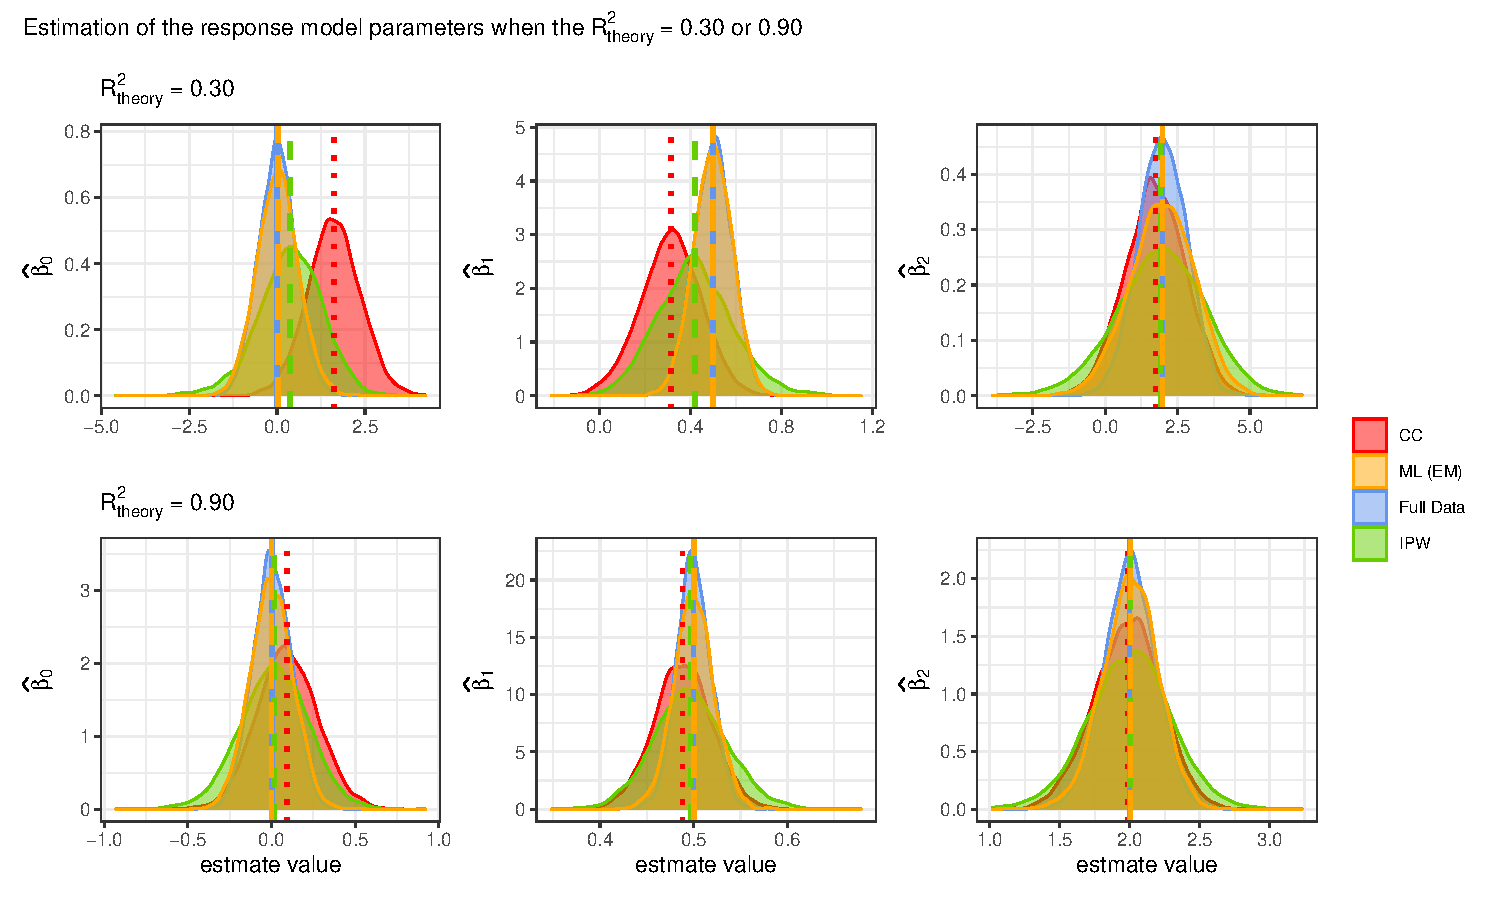
\includegraphics{sampldist-1} 

}

\caption{Density plots of the simulation results for estimating the parameters in the linear model $Y_i = \beta_0 + \beta_1 X_i + \beta_2 Z_i + \epsilon_i$, where $i = 1,...,100$, $X_i \overset{IID}{\sim} N(0, \phi^2)$, $Z_i \overset{IID}{\sim} Bernoulli(\theta)$, and $\epsilon_i \overset{IID}{\sim} N(0, \sigma^2)$. The true parameters values are $(\theta, \phi, \beta_0, \beta_1, \beta_2) = (0.4, 5, 0, 0.5, 2)$, $(\gamma_0, \gamma_1, \gamma_2) = (1, 1, 1)$, $R_{\mathrm{latent}}^2 = 0.60$ and $R_{\mathrm{theory}}^2 = 0.30 \text{ or } 0.90$. The vertical lines represent the sample mean of the estimates over 5,000 replications.}\label{fig:sampldist}
\end{figure}

\begin{table}[H]

\caption{\label{tab:unnamed-chunk-1}Simulation results of estimating the parameters in the linear model $Y_i = \beta_0 + \beta_1 X_i + \beta_2 Z_i + \epsilon_i$, where $i = 1,...,100$, $X_i \overset{IID}{\sim} N(0, \phi^2)$, $Z_i \overset{IID}{\sim} Bernoulli(\theta)$, and $\epsilon_i \overset{IID}{\sim} N(0, \sigma^2)$. The true parameters values are $(\theta, \phi, \beta_0, \beta_1, \beta_2) = (0.4, 5, 0, 0.5, 2)$, $(\gamma_0, \gamma_1, \gamma_2) = (1, 1, 1)$, $R_{\mathrm{latent}}^2 = 0.60$ and $R_{\mathrm{theory}}^2 = 0.30 \text{ or } 0.90$. Results in the first column are calculated using the full data set. Results in the last three columns are based on the ODS data set. They are from the complete case analysis, from IPW with 20 as the truncation bound, and from the maximum likelihood method using the EM algorithm. In each row group, the first row contains the sample means of the estimates over 5,000 replications, the second row contains the sample standard deviation, and the third row contains the coverage rate, the proportion of the 95 percent CIs capturing the true parameter}
\centering
\begin{tabular}[t]{rrrrr}
\toprule
\multicolumn{2}{c}{ } & \multicolumn{3}{c}{Analysis Methods} \\
\cmidrule(l{3pt}r{3pt}){3-5}
$R_{\mathrm{theory}}^{2}$ & Full Data & CC & IPW & ML (EM)\\
\midrule
\addlinespace[0.3em]
\multicolumn{5}{l}{\textbf{$\beta_0 = 0$}}\\
\hspace{1em}0.3 & 0.000 & 1.615 & 0.368 & 0.021\\
\hspace{1em} & 0.526 & 0.753 & 0.929 & 0.595\\
\hspace{1em} & 0.951 & 0.430 & 0.823 & 0.951\\
\hspace{1em}0.9 & 0.003 & 0.093 & 0.015 & 0.000\\
\hspace{1em} & 0.115 & 0.181 & 0.206 & 0.128\\
\hspace{1em} & 0.949 & 0.913 & 0.855 & 0.948\\
\addlinespace[0.3em]
\multicolumn{5}{l}{\textbf{$\beta_1 = 0.5$}}\\
\hspace{1em}0.3 & 0.499 & 0.314 & 0.420 & 0.499\\
\hspace{1em} & 0.084 & 0.133 & 0.167 & 0.085\\
\hspace{1em} & 0.948 & 0.673 & 0.781 & 0.950\\
\hspace{1em}0.9 & 0.500 & 0.488 & 0.497 & 0.500\\
\hspace{1em} & 0.018 & 0.031 & 0.039 & 0.022\\
\hspace{1em} & 0.948 & 0.925 & 0.810 & 0.948\\
\addlinespace[0.3em]
\multicolumn{5}{l}{\textbf{$\beta_2 = 2$}}\\
\hspace{1em}0.3 & 1.980 & 1.732 & 1.911 & 1.970\\
\hspace{1em} & 0.831 & 1.034 & 1.523 & 1.126\\
\hspace{1em} & 0.953 & 0.943 & 0.845 & 0.950\\
\hspace{1em}0.9 & 2.000 & 1.985 & 2.001 & 2.004\\
\hspace{1em} & 0.186 & 0.240 & 0.296 & 0.199\\
\hspace{1em} & 0.945 & 0.947 & 0.887 & 0.948\\
\bottomrule
\end{tabular}
\end{table}

\hypertarget{model-misspecifications-influence-on-estimators}{%
\subsubsection{5.3 Model Misspecification's Influence on
Estimators}\label{model-misspecifications-influence-on-estimators}}

We augmented the above simulations to assess response model
misspecification's impact on the estimators. The same linear analysis
model is used for each estimator. However, to test estimators'
performance under the circumstance of mean model misspecification, we
altered the response model in data generation: \[
Y_i = \beta_0 + \beta_1 X_i^{\bullet} + \beta_2 Z_i + \epsilon_i
\] where \(X_i^{\bullet}\) is a nonlinear function of \(X_i\). Thus, we
misspecify the model if we assume \(Y\) has a linear relationship with
\(X\). The goal is to test whether the estimators yield reliable
estimates for \(\beta_2\) even if we make an incorrect assumption about
the relationship between \(Y\) and \(X\). We have to notice that the
only thing that changes in this setting is the relation between \(X\)
and \(Y\) in data generation. Both variables are collected in the final
simulated data set. \(X^{\bullet}\) is a latent auxiliary variable. It
implies we will have a model misspecification issue if we use the
original response mean model. To control the degree of misspecification,
we define \(X_i^{\bullet}\) as follows. \[
X_i^{\bullet} = \kappa \cdot X_i(X_i - \phi)(X_i + \phi) + X_i
\] where \(\phi\) is the population standard deviation of \(X_i\) and
\(\kappa\) is the misspecification level. We can use any value in the
place of \(\phi\), but using \(\phi\) ensures the simulated data are
scattered within a reasonable range. Here, \(\kappa\) is used to
quantify the level of misspecification. If \(\kappa\) is a small value,
the nonlinear portion in \(X_i^{\bullet}\) is negligible. Then, the
simulated data set in the model misspecification setting will be similar
to the one generated using the original setting, and the analysis
results will generally be the same. However, if \(\kappa\) is a large
value, the simulated data and analysis result will be significantly
different. Therefore, we compare the estimators' performance under
varied \(\kappa\).

When the analysis model is misspecified, all estimators tend to be
unstable and yield estimates with high standard error. The high
variability leads to a high coverage rate for \(\hat\beta_2\) in all
three methods, but the value is meaningless. The estimates can have an
enormous bias, but the even larger standard error helps to construct
wide CIs to cover the true value. Therefore, we utilize mean squared
error (MSE) as the metric to compare estimators' efficiency. MSE
captures both the bias and variance of the estimate. A lower MSE
indicates better efficiency.

We generate 5,000 replications of random full data sets and their
corresponding ODS-designed data sets for the model misspecification
scenario. We set \(N = 100\),
\((\theta, \phi, \beta_0, \beta_1, \beta_2) = (0.5, 5, 0, 0.5, 2)\),
\((\gamma_1, \gamma_2, \gamma_3) = (1, 1, 1)\), and
\(R_{\mathrm{latent}}^2 = 0.60\). We choose two values for
\(R_{\mathrm{theory}}^2\): 0.30 and 0.90, and three values for
\(\kappa\): 0.01, 0.1, and 1. For each pair of \(R_{\mathrm{theory}}^2\)
and \(\kappa\), we perform a simulation study with the above setting.
The goal of interest is to study if the incorrect assumption of the
relationship between \(X\) and \(Y\) can affect the estimation of
\(\beta_2\). Thus, we compare the estimators only with respect to
\(\hat{\beta_2}\). In Tables 3 and 4, the first column lists the results
of estimating \(\beta_2\) using the least-squares estimator with all the
observations in the full data set. The other three columns list the
results of estimating the parameter using different analysis methods
with the ODS-designed data set. The second column lists the results of
the CC analysis, the third column lists the results of the IPW method,
and the fourth column lists the results of the ML method using the EM
algorithm. We calculate the sample mean of
\(\mathrm{MSE}(\hat{\beta_2})\) over the 5,000 iteration. It can easily
proven that
\(\mathrm{MSE}(\hat{\beta_2}) = \mathrm{Bias}^{2}(\hat{\beta_2}) + \mathrm{Var}(\hat{\beta_2})\).

\begin{table}[H]

\caption{\label{tab:unnamed-chunk-2}Simulation results of estimating only $\beta_2$ when $R_{\mathrm{theory}}^2 = 0.30 \text{ or } 0.90$, where both model well-specified scenario and model misspecified scenarios are included. The value of the parameter is 2. The four columns list the results from different analysis methods. Results in the first column are calculated using the full data set. Results in the last three columns are based on the ODS data set. They are from the complete case analysis, from IPW with 20 as the truncation bound, and from the maximum likelihood method using the EM algorithm. In each row group, the first row contains the sample means of $\hat{\beta_2}$ over 5,000 replications, the second row contains the of $\mathrm{MSE}(\hat{\beta_2})$.}
\centering
\begin{tabular}[t]{rrrrr}
\toprule
\multicolumn{5}{c}{$\beta_2$ = 2} \\
\cmidrule(l{3pt}r{3pt}){1-5}
\multicolumn{2}{c}{ } & \multicolumn{3}{c}{Analysis Methods} \\
\cmidrule(l{3pt}r{3pt}){3-5}
$R_{\mathrm{theory}}^{2}$ & Full Data & CC & IPW & ML (EM)\\
\midrule
\addlinespace[0.3em]
\multicolumn{5}{l}{\textbf{Correctly Specified}}\\
\hspace{1em}0.3 & 1.980 & 1.732 & 1.911 & 1.970\\
\hspace{1em} & 0.691 & 1.141 & 2.326 & 1.269\\
\hspace{1em}0.9 & 2.000 & 1.984 & 2.001 & 2.003\\
\hspace{1em} & 0.034 & 0.058 & 0.087 & 0.040\\
\addlinespace[0.3em]
\multicolumn{5}{l}{\textbf{Misspecified, $\kappa$ = 0.01}}\\
\hspace{1em}0.3 & 1.984 & 1.802 & 1.972 & 1.964\\
\hspace{1em} & 0.805 & 1.360 & 2.306 & 1.440\\
\hspace{1em}0.9 & 1.996 & 2.021 & 1.999 & 1.902\\
\hspace{1em} & 0.131 & 0.208 & 0.179 & 0.178\\
\addlinespace[0.3em]
\multicolumn{5}{l}{\textbf{Misspecified, $\kappa$ = 0.1}}\\
\hspace{1em}0.3 & 1.968 & 1.885 & 1.991 & 1.713\\
\hspace{1em} & 10.006 & 17.213 & 10.407 & 14.950\\
\hspace{1em}0.9 & 2.014 & 2.036 & 2.073 & 1.888\\
\hspace{1em} & 9.542 & 16.733 & 8.796 & 14.386\\
\addlinespace[0.3em]
\multicolumn{5}{l}{\textbf{Misspecified, $\kappa$ = 1}}\\
\hspace{1em}0.3 & 2.413 & 2.816 & 2.853 & 0.760\\
\hspace{1em} & 959.492 & 1832.761 & 932.155 & 1521.635\\
\hspace{1em}0.9 & 2.261 & 2.706 & 2.585 & 0.513\\
\hspace{1em} & 972.835 & 1946.229 & 985.904 & 1594.518\\
\bottomrule
\end{tabular}
\end{table}

The results in Tables 2 allow a discussion about how the
misspecification influences various estimators from two aspects: bias,
efficiency. When \(R_{\mathrm{theory}}^{2} = 0.30\) and
\(\kappa = 0.01\), the misspecification has negligible effect on three
estimators' performance. The CC estimator gives the most biased
estimate, but it tends to be more efficient than the other estimators
under the MSE criterion. IPW estimator is less biased, but it is more
unstable and inefficient than other estimators. ML estimator is less
biased than the CC estimator, and it is more stable and efficient than
the IPW estimator. However, when the degree of misspecification becomes
more significant, \(\kappa = 0.1\), all three estimators receive
different levels of influence. The IPW estimator becomes the most
unbiased, stable, and efficient estimator among the three. On the
contrary, the CC estimator becomes more unstable than IPW, and the ML
estimator becomes the most biased and inefficient. When \(\kappa = 1\),
all three estimators become highly biased and inefficient, but the IPW
estimator remains the most unbiased and efficient among them. When
\(R_{\mathrm{theory}}^{2} = 0.90\) and \(\kappa = 0.01\), all three
estimators are unbiased and efficient. Similarly, all estimators receive
varied levels of impact as the response model becomes more misspecified.
The IPW estimator receives the least effect, while the ML estimator is
the most vulnerable to model misspecification.

\hypertarget{discussion}{%
\subsection{6 Discussion}\label{discussion}}

Our simulation results corroborate the results from the previous work.
In an ODS study, CC analysis can be reliable only when the response
variable has a strong relationship with the predictor variables. The ML
method achieves its ideal performance when our assumption about the
response model is valid. Once the assumption is incorrect, the estimator
can be highly biased and inefficient since the EM algorithm is
sensitive. Moreover, no software package supports the EM algorithm by
default, and the development of the algorithm requires a considerable
amount of time and effort. On the other hand, the IPW approach, although
not ideally unbiased and efficient as the ML method, is easy to
implement in many software packages. Therefore, from our limited
experience, we make the following recommendations. Unless there is
evidence that the response variable has a perfect relationship with the
predictor variables, CC analysis does not correctly address the
missingness. Instead, IPW can be used as an improvised method. After
thoroughly learning the data set, we can use the ML method and develop
an EM algorithm to calculate the estimates.

Several extensions of the design and methods are worth mentioning. The
first extension is to compare and contrast IPW and EM estimators'
efficiency using bootstrapping. The case resampling process must be
stratified to maintain the degree of missingness in each bootstrapped
data set. Another extension is to explore the poor coverage rate of the
IPW estimator. In our simulation results, the 95 percent CI coverage
rates of the IPW estimates do not fall into \([0.936, 0.964]\). However,
Weaver and Zhou (2005) have the IPW estimators achieve reasonable
coverage rates in their ODS design. The reason for the difference is
that the IPW estimates standard errors we use are directly from the
software package by default, which is commonly used in practice.
However, these values are not theoretically correct. Therefore, we need
to develop our own functions to compute the theoretical standard errors.

\hypertarget{appendix}{%
\subsection{Appendix}\label{appendix}}

In our ODS design, we have the following setup \[
\begin{aligned}
y_i | x_i, z_i &\overset{Ind}{\sim} N(\beta_0 + \beta_1 x_i + \beta_2 z_i, \sigma^2) \\
x_i &\overset{IID}{\sim} N(0, \phi^2) \\
z_i &\overset{IID}{\sim} Bernoulli(\theta) \\
R_i &= \mathbb{I}(z_i \text{ is observed}) \\
\end{aligned}
\]

The observed likelihood is \[
L_{Obs}(\boldsymbol\Theta) = \prod_{i=1}^{N} \big[ f(y_i, x_i; \boldsymbol\Theta)f(z_i|y_i, x_i; \boldsymbol\Theta) \big]^{R_i} \big[ f(y_i, x_i; \boldsymbol\Theta) \big]^{1-R_i}
\] We also know the complete likelihood is \[
\begin{aligned}
L(\boldsymbol\Theta) 
&= f(\boldsymbol{y}, \boldsymbol{x}, \boldsymbol{z}_{S}, \boldsymbol{z}_{\bar{S}}; \boldsymbol{\Theta}) \\
&= \prod_{i=1}^{N} f(z_i|y_i, x_i; \boldsymbol\Theta)f(y_i, x_i; \boldsymbol\Theta) \\
\end{aligned}
\] Then, the conditional likelihood of \(\boldsymbol{z}_{\bar{S}}\)
given all the observed data is \[
\begin{aligned}
f(\boldsymbol{z}_{\bar{S}} | \boldsymbol{y}, \boldsymbol{x}, \boldsymbol{z}_{S}; \boldsymbol{\Theta}) 
&= \frac{f(\boldsymbol{y}, \boldsymbol{x}, \boldsymbol{z}_{S}, \boldsymbol{z}_{\bar{S}}; \boldsymbol{\Theta})}{f(\boldsymbol{y}, \boldsymbol{x}, \boldsymbol{z}_{S}; \boldsymbol{\Theta})} \\
&= \frac{L(\boldsymbol\Theta)}{L_{Obs}(\boldsymbol\Theta)} \\
&= \prod_{i=1}^{N} \big[ f(z_i | y_i, x_i) \big]^{1-R_i}
\end{aligned}
\]

Note that \(L(\boldsymbol{\Theta})\) can also be expressed as
\(f(\boldsymbol{y}|\boldsymbol{x},\boldsymbol{z})f(\boldsymbol{x})f(\boldsymbol{z})\).

\hypertarget{expectation-step}{%
\subsubsection{Expectation Step}\label{expectation-step}}

By definition, \[
Q(\boldsymbol{\Theta} | \hat{\boldsymbol{\Theta}}^{(m)}) = \mathrm{E}[\log L(\boldsymbol\Theta)]
\] where the expectation is over
\(f(\boldsymbol{z}_{\bar{S}} | \boldsymbol{y}, \boldsymbol{x}, \boldsymbol{z}_{S}; \boldsymbol{\Theta})\).
Thus, due to the independence among all observations, the \(Q\) function
can be expressed as follows: \[
\begin{aligned}
Q(\boldsymbol{\Theta} | \hat{\boldsymbol{\Theta}}^{(m)}) &= \sum_{i = 1}^{N} \Big( 
R_i \log f(y_i|x_i, z_i) + (1 - R_i) \cdot \mathrm{E}[\log f(y_i|x_i, z_i)] \\
&+ \log f(x_i) + 
R_i \log f(z_i) + (1 - R_i) \cdot \mathrm{E}[\log f(z_i)]
\Big)
\end{aligned}
\] where \(x_i\)'s distribution parameters does not affect the
estimation for \(\boldsymbol{\beta}\) so that \(\log f(x_i)\) can be
ignored in the future calculation.

We can prove that \[
f(y_i, x_i) = f(y_i|x_i, z_i = 0) f(x_i) (1 - \theta) + f(y_i | x_i, z_i = 1) f(x_i) \theta
\] and \[
\begin{aligned}
z_i | y_i, x_i &\overset{Ind}{\sim} Bernoulli (\phi^{\prime}_i), \forall i \in \bar{S} \\
\\
\text{where } \phi^{\prime}_i &= \frac{f(y_i|x_i, z_i = 1)\theta}{f(y_i|x_i, z_i = 1)\theta + f(y_i|x_i, z_i = 0)(1 - \theta)}
\end{aligned}
\]

Therefore, we can express the \(Q\) function as follows: \[
\begin{aligned}
Q(\boldsymbol{\Theta} | \hat{\boldsymbol{\Theta}}^{(m)}) &= \sum_{i = 1}^{N} \Big[
R_i \log f(y_i | x_i, z_i) + R_i \log f(z_i) \\
&+ (1-R_i) \log f(y_i | x_i, z_i = 1) \phi_i^{\prime} + (1-R_i) \log f(y_i | x_i, z_i = 0) (1- \phi_i^{\prime}) \\
&+ (1-R_i)\big( \phi_i^{\prime} \log(\theta) + (1-\phi_i^{\prime}) \log(1 - \theta) \big) \Big] 
\end{aligned}
\] which is iteratively maximized during the maximization step.

\hypertarget{maximization-step}{%
\subsubsection{Maximization Step}\label{maximization-step}}

In this step, we iteratively maximize the \(Q\) function by letting \[
\hat{\boldsymbol{\Theta}}^{(m+1)} =  \operatorname*{arg\,max} Q(\boldsymbol{\Theta} | \hat{\boldsymbol{\Theta}}^{(m)})
\]

\(Q(\boldsymbol{\Theta} | \hat{\boldsymbol{\Theta}}^{(m)})\) can be
decomposed as follows: \[
Q(\boldsymbol{\Theta} | \hat{\boldsymbol{\Theta}}^{(m)}) = Q_{\theta} + Q_{\boldsymbol\beta, \sigma^2}
\] \[
Q_{\theta} = \sum_{i=1}^{N} R_i \log f(z_i) + \sum_{i=1}^{N} (1 - R_i) \big( \phi_i^{\prime} \log(\theta) + (1 - \phi_i^{\prime}) \log(1 - \theta) \big)
\] \[
\begin{aligned}
Q_{\boldsymbol\beta, \sigma^2} &= \sum_{i=1}^{N} R_i \log f(y_i|x_i, z_i) + \sum_{i=1}^{N} \log f(y_i|x_i, z_i = 0)(1 - \phi_i^{\prime}) \\
&+ \sum_{i=1}^{N}(1 - R_i) \log f(y_i|x_i, z_i = 1)\phi_i^{\prime}
\end{aligned}
\]

Then, we can maximize the estimates element-wisely.

For \(\theta\), we can directly calculate the updated estimate by
setting \(\frac{d}{d\theta}Q_{\theta} = 0\). For \(\boldsymbol\beta\)
and \(\sigma^2\), we can use the default weighted least-squares
estimation in many software packages. It can be derived that \[
Q_{\boldsymbol\beta, \sigma^2} = - \frac{n}{2} \log(2\pi\sigma^2) - \frac{S(\boldsymbol\beta)}{2\sigma^2}
\] where \[
\begin{aligned}
S(\boldsymbol\beta) &= \sum_{i = 1}^{N} \Big(
R_i(y_i - \beta_0 - \beta_1 x_i - \beta_2 z_i)^2 + (1 - R_i)\big(
    (y_i - \beta_0 - \beta_1 x_i - \beta_2)^2 \phi_i^{\prime} \\
    &+ (y_i - \beta_0 - \beta_1 x_i)^2 (1 - \phi_i^{\prime})
  \big)
\Big)
\end{aligned}
\]

The updated estimate for \(\boldsymbol\beta\) is calculated by \[
\operatorname*{arg\,max}_{\boldsymbol\beta} Q_{\boldsymbol\beta, \sigma^2} = \operatorname*{arg\,min}_{\boldsymbol\beta} S(\boldsymbol\beta)
\] which is essentially the weighted least-square estimator of an
auxiliary data set. The auxiliary data set consists of three components:
the complete cases, the incomplete cases with \(z_i\)'s imputed as 1,
and the incomplete cases with \(z_i\)'s imputed as 0. After obtaining
the updated estimate for \(\boldsymbol\beta\), we can calculate the
updated estimate of \(\sigma^2\) by setting
\(\frac{d}{d\theta}Q_{\boldsymbol\beta, \sigma^2} = 0\). It is
noteworthy that we also need to update \(\phi_i^{\prime}\)'s during each
iteration.

The algorithm terminates when the minimum change in the estimates,
\(\min(d \hat{\boldsymbol{\Theta}})\), is less than a tolerance value.

\hypertarget{reference}{%
\subsection*{Reference}\label{reference}}
\addcontentsline{toc}{subsection}{Reference}

\hypertarget{refs}{}
\begin{CSLReferences}{1}{0}
\leavevmode\vadjust pre{\hypertarget{ref-schafer}{}}%
Schafer, Joseph L, and John W Graham. 2002. {``Missing Data: Our View of
the State of the Art.''} \emph{Psychological Methods} 7 (2): 147.

\leavevmode\vadjust pre{\hypertarget{ref-seaman}{}}%
Seaman, Shaun R, and Ian R White. 2013. {``Review of Inverse Probability
Weighting for Dealing with Missing Data.''} \emph{Statistical Methods in
Medical Research} 22 (3): 278--95.

\leavevmode\vadjust pre{\hypertarget{ref-weaver}{}}%
Weaver, Mark A, and Haibo Zhou. 2005. {``An Estimated Likelihood Method
for Continuous Outcome Regression Models with Outcome-Dependent
Sampling.''} \emph{Journal of the American Statistical Association} 100
(470): 459--69.

\leavevmode\vadjust pre{\hypertarget{ref-white}{}}%
White, Ian R, and John B Carlin. 2010. {``Bias and Efficiency of
Multiple Imputation Compared with Complete-Case Analysis for Missing
Covariate Values.''} \emph{Statistics in Medicine} 29 (28): 2920--31.

\leavevmode\vadjust pre{\hypertarget{ref-zhao}{}}%
Zhao, LP, and S Lipsitz. 1992. {``Designs and Analysis of Two-Stage
Studies.''} \emph{Statistics in Medicine} 11 (6): 769--82.

\end{CSLReferences}

\end{document}
